\subsection{Petri net editor}
\writer{Albert}

The Petri net editor is a component which consists of an extension of the ePNK editor. It contains all the functionality that ePNK provides and also adds the features described previously in this document, and that can be summarized in Figure \ref{fig:uml-petrinet-editor}. Its actual implementation is shown in Figure \ref{fig:petri-net-domain-model}.

\begin{figure}[htp]
\begin{center}
  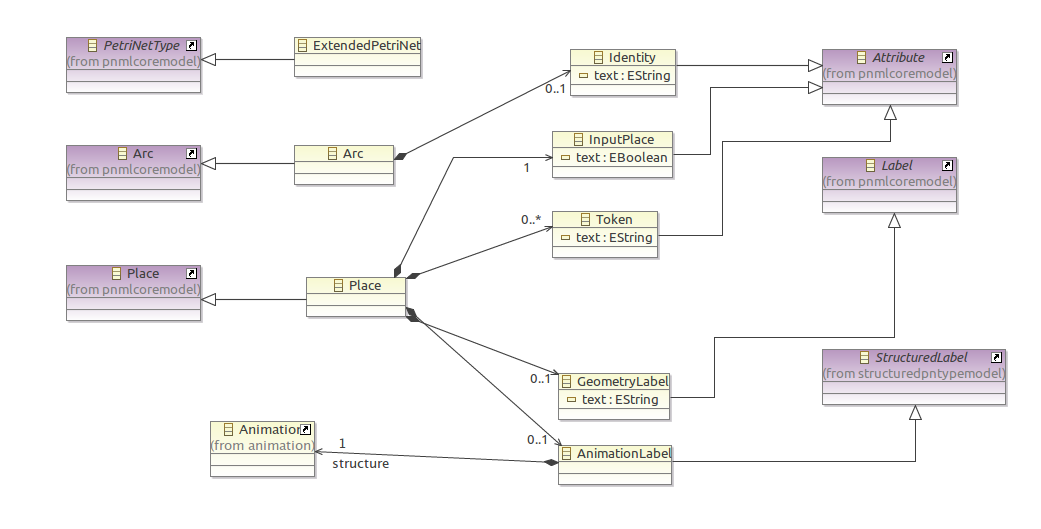
\includegraphics[width=0.8\textwidth]{image/petrinet_editor_domain.png}
  \caption{Petri net editor domain model}
  \label{fig:petri-net-domain-model}
\end{center}
\end{figure}

\subsubsection{Petri net editor classes}

A description of the classes shown in Figure \ref{fig:petri-net-domain-model} is provided.

\paragraph{Place}

The class Place extends from Place in the \textit{pnmlcoremodel}, and contains the following attributes:

\begin{itemize}
	\item \textbf{Token}: an ePNK label to indicate the presence of one or more tokens in this Place.
	\item \textbf{InputPlaceLabel}: an ePNK boolean attribute to indicate if the place is interactive for the user or not (if tokens can be added by the user during runtime ).
	\item \textbf{GeometryLabel}: an ePNK string label to indicate the geometry location of the Place in the simulation.
	\item \textbf{AnimationLabel}: : an ePNK structured label which contains an Animation object and that contains all the information of the animation or sequence of animations executed when a Token is in this Place.
\end{itemize}

\subsubsection{Animation}

As shown in Figure~\ref{fig:petri-net-domain-model}, Places have a defined animation model, which is the one shown in Figure~\ref{fig:animation-model}.

\begin{figure}[htp]
\begin{center}
  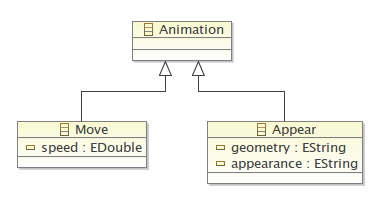
\includegraphics[width=0.5\textwidth]{image/animation_model.png}
  \caption{Animation model}
  \label{fig:animation-model}
\end{center}
\end{figure}

As shown, there are two possible animations: move or appear. The first one also has speed as a parameter, whilst the second one includes the geometry label of the place of which we want to change the shape on, and the shape we want that place to have. Using this two animations, it is possible to visualize all the necessary animations.

\subsubsection{PAL: Petri Net Animation Language}

In order to be able to read the animations defined in an animation label in the Petri Net Editor, it has been implemented a language using Xtext. The defined syntax is the following:

\begin{lstlisting}
	move(2.0)
\end{lstlisting}

\begin{lstlisting}
	appear(L1, red)
\end{lstlisting}

\subsubsection{Graphical Extensions}

When extending from the ePNK it has been also necessary to add two graphical extensions in order to provide more usability to the end-user by letting him know in a single look which places have tokens and which are input places. Therefore, we implemented the following method in an inherited class of PlaceFigure, which depending on Place having tokens or having been marked as input place, the shape would change on run time.
\begin{lstlisting}
protected void fillShape(Graphics graphics) {
		super.fillShape(graphics);
		dk.dtu.se2.petrinet.Place p = (dk.dtu.se2.petrinet.Place) this.place;
		
		if (!p.getTokens().isEmpty()) {
			Rectangle rectangle = this.getClientArea();
			graphics.setBackgroundColor(getForegroundColor());
			graphics.fillOval((int) (rectangle.x + 0.325 * rectangle.width), 
					(int) (rectangle.y + 0.375 * rectangle.height),
					(int) (0.25 * rectangle.width), (int) (0.25 * rectangle.height));
			graphics.drawString(String.valueOf(p.getTokens().size()), 
					(int) (rectangle.x + 0.6 * rectangle.width), 
					(int) (rectangle.y + 0.45 * rectangle.height));
		}
		
		InputPlace inputPlace = p.getInputPlaceLabel();
		if(inputPlace != null && inputPlace.isText()){
			Rectangle rectangle = this.getClientArea();
			graphics.setBackgroundColor(getForegroundColor());
			graphics.setLineWidth(2);
			graphics.drawLine(rectangle.x + 10, rectangle.y + 10, 
					rectangle.x + rectangle.width - 10, rectangle.y + rectangle.height - 10);
			graphics.drawLine(rectangle.x + 10, rectangle.y + rectangle.height - 10, 
					rectangle.x + rectangle.width - 10, rectangle.y + 10);
		}
	}
\end{lstlisting}